\section{Dataset Analysis}

\subsection{Dataset}
The dataset provided is comprised of 803 days of visits measurements from 145063 combination of wikipedia page and access agent. An page name and header example can be seen on table \ref{tab:wiki_data}. The entries with NaN are correspondent to the days when the wikipedia page did not existed yet, thus those values where substituted by 0 in order to treat this edge case.

\begin{table}[htbp]
\centering
	\begin{tabular}{|c|c|c|c|c|c|}\hline
		&2015&2015&2015&2015&2015\\
		&07/01&07/02&07/03&07/04&07/05\\\hline
		2NE1\_zh.wikipedia.org\_all...& 18  key& 11  & 5   & 13  & 14 \\\hline
		2PM\_zh.wikipedia.org\_all-...& 11  & 14  & 15  & 18  & 11 \\\hline
		3C\_zh.wikipedia.org\_all-a...& 1   & 0   & 1   & 1   & 0 \\ \hline
		4minute\_zh.wikipedia.org\_...& 35  & 13  & 10  & 94  & 4 \\\hline
		52\_Hz\_I\_Love\_You\_zh.wi...& NaN & NaN & NaN & NaN & NaN \\\hline
		5566\_zh.wikipedia.org\_al-...& 12 & 7 & 4 & 5 & 20 \\\hline
		91Days\_zh.wikipedia.org\_a...&NaN&NaN&NaN&NaN&NaN \\\hline
		A'N'D\_zh.wikipedia.org\_al...& 118 & 26 & 30 & 24 & 29\\\hline
	\end{tabular}
	\vspace{1mm}
		\caption{Data Example from kaggle series forecast\label{tab:wiki_data}}
\end{table}


The first step was performing an analysis of the data to understand which patterns could leverage our learning methods. Plotting graphs of the traffic from a few pages we observed that different pages show remarkably distinguish trends in traffic. This suggests that a good model needs to explicitly differentiate pages.
For specific entries we note a strong year-to-year autocorrelation. We also observed weaker week-to-week and month-to-month trends. One clear example of this case was the Thanksgiving holiday page that showed an yearly spike around a Thursday on late November, which is the day of the holiday.

\begin{figure}[h!]
  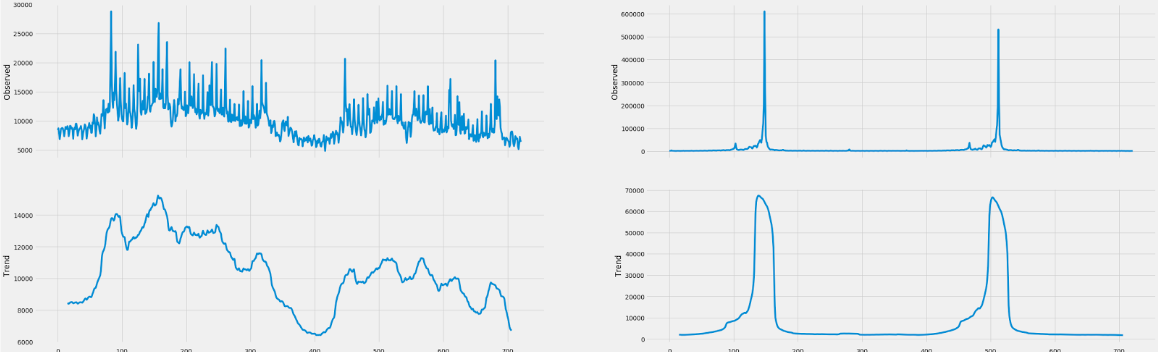
\includegraphics[width=\linewidth]{analysis1.png}
  \caption{Observed Traffic and Traffic Trend from two different pages}
  \label{fig:analysis1}
\end{figure}

\begin{figure}[h!]
	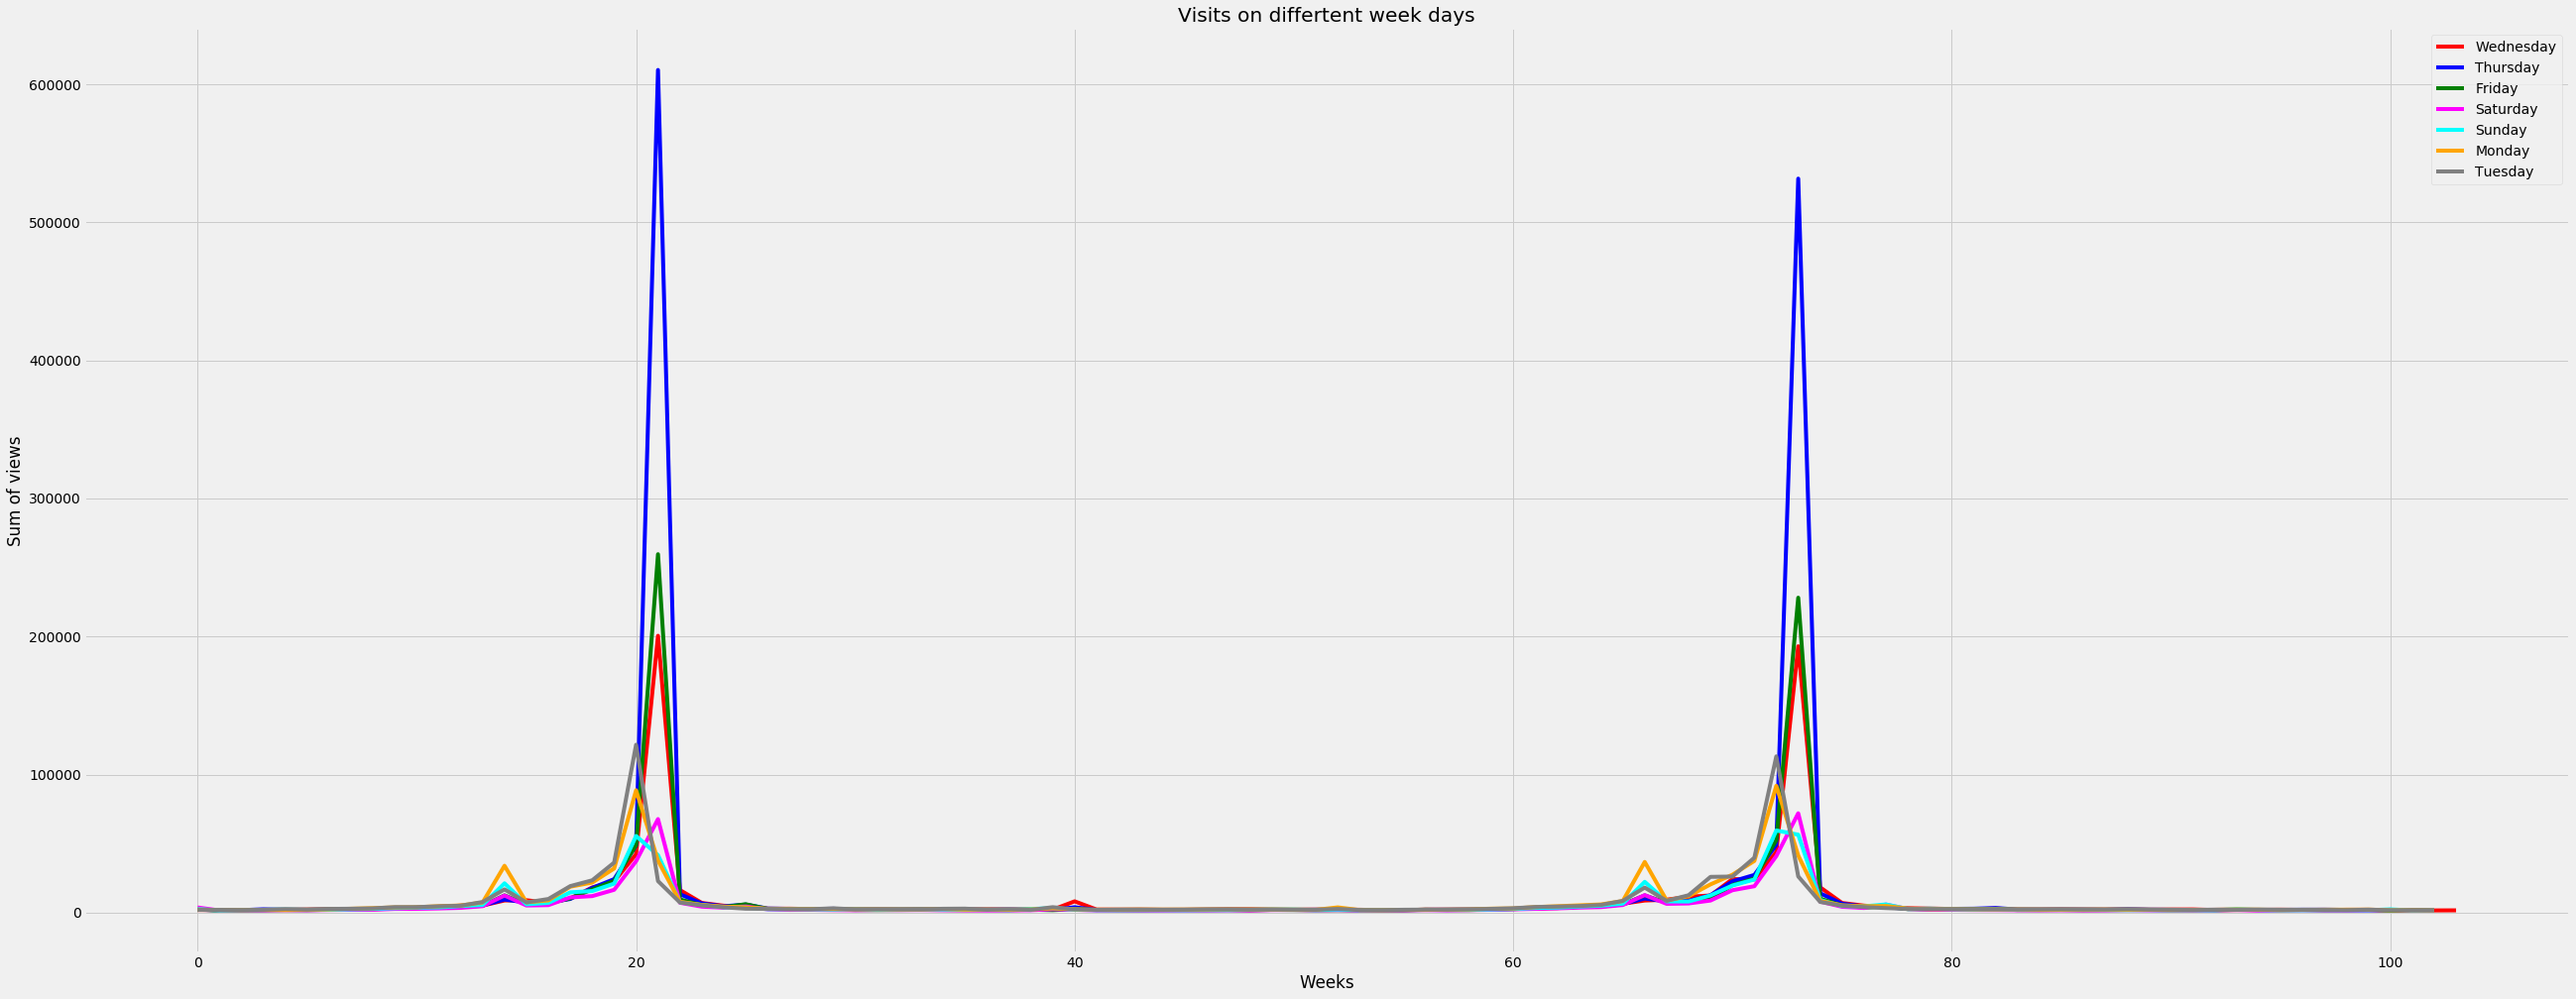
\includegraphics[width=\linewidth]{weekly_TK.png}
	\caption{Observed Traffic separated by weekday for the thanksgiving page.}
	\label{fig:thanksgiving}
\end{figure}

Additionally, we have to deal with spikes in traffic not following a regular pattern. We note a short-term dependency following those spikes, which means the days immediately before the prediction are important to consider.


